%------------------------------------------%
% Cannabis Data Science
% Date: 2/16/2022
%------------------------------------------%
\documentclass[xcolor={dvipsnames}]{beamer}
\hypersetup{pdfpagemode = FullScreen}
\mode<presentation>{
  \usetheme{Boadilla}
  \usecolortheme{orchid}
  \usefonttheme{default}
  \setbeamertemplate{navigation symbols}{}
  \setbeamertemplate{caption}[numbered]
}
\setbeamersize{
  text margin left = 0.5in,
  text margin right = 0.5in
}

%------------------------------------------%
% Title
%------------------------------------------%
\title[\textbf{Cannabis Data Science \#53}]{}
\author{Cannabis Data Science}
\institute[]{\Large Cannabis Data Science \#53}
\date{February \nth{16}, 2022}

%------------------------------------------%
% Packages
%------------------------------------------%
\usepackage[english]{babel}
\usepackage[utf8x]{inputenc}
\usepackage{tikz} % For styling.
\usepackage{xparse}

%------------------------------------------%
% Colors
%------------------------------------------%
%\usepackage[dvipsnames]{xcolor}
\definecolor{Green}{RGB}{34, 153, 84}
\definecolor{LightGreen}{RGB}{218, 247, 166}
\definecolor{DarkGreen}{RGB}{2, 48, 32}
\definecolor{Orange}{RGB}{255, 87, 51}
\definecolor{DarkOrange}{RGB}{199, 0, 57}
\definecolor{Yellow}{RGB}{255, 195, 0}

%------------------------------------------%
% Theme
%------------------------------------------%
\setbeamercolor*{palette primary}{bg=LightGreen, fg=DarkGreen}
\setbeamercolor*{palette secondary}{bg=LightGreen, fg=DarkGreen}
\setbeamercolor*{palette tertiary}{bg=LightGreen, fg=DarkGreen}
%\setbeamercolor*{palette quaternary}{bg=myNewColorD, fg = green}

%------------------------------------------%
% Packages
%------------------------------------------%
\usepackage{amsmath}
\renewcommand*\footnoterule{} % No separating line on footnote.
\usepackage{mathtools} % For annotating equations.
\usepackage{hhline} % for double bars.
\usepackage[super]{nth} % For formatting 1st, 2nd, 3rd, etc.
\usepackage{graphicx, caption, subcaption}

%------------------------------------------%
% Commands
%------------------------------------------%

% Top space.
\newcommand\T{\rule{0pt}{2.5ex}}

% Bottom space.
\newcommand\B{\rule[-1.25ex]{0pt}{0pt}}

% Blocks.
\newenvironment<>{Block}[2][.9\textwidth]
  {\setlength{\textwidth}{#1}
  \begin{actionenv}#3
    \def\insertblocktitle{#2}\par
    \usebeamertemplate{block begin}}
  {\par\usebeamertemplate{block end}
  \end{actionenv}}

% Balls.
\defbeamertemplate{enumerate item}{largeball}
{\begin{pgfpicture}{-1ex}{-0.65ex}{1.5ex}{1.5ex}
\usebeamercolor[fg]{item projected}
{\pgftransformscale{2.5}\pgftext{\Large\pgfuseshading{bigsphere}}}
{\pgftransformshift{\pgfpoint{0pt}{0.5pt}}
\pgftext{\usebeamerfont*{item projected}\small\insertenumlabel}}
\end{pgfpicture}}

% Fancy arrows.
\NewDocumentCommand\UpArrow{O{2.0ex} O{black}}{%
   \mathrel{\tikz[baseline] \draw [->, line width=0.5pt, #2] (0,0) -- ++(0,#1);}} % Fancy up-arrow.
\NewDocumentCommand\DownArrow{O{2.0ex} O{black}}{%
   \mathrel{\tikz[baseline] \draw [<-, line width=0.5pt, #2] (0,0) -- ++(0,#1);}} % Fancy down-arrow.

% Equations with numbers on the left.
\makeatletter
\newcommand{\LeftEqNo}{\let\veqno\@@leqno}
\makeatother

%------------------------------------------%
% Presentation
%------------------------------------------%
\begin{document}

% Title page.
\begin{frame}{}
  
\includegraphics[scale=0.33]{images/logo.pdf}
  \vspace*{-2\baselineskip}
  \titlepage
\end{frame}

%------------------------------------------%
% Introduction
%------------------------------------------%
\section{Introduction}

\begin{frame}{}

% Figures
{\large \textbf{We've visualized the supply side in prior weeks:}}\\
\begin{minipage}{.5\textwidth}
  \begin{figure}
    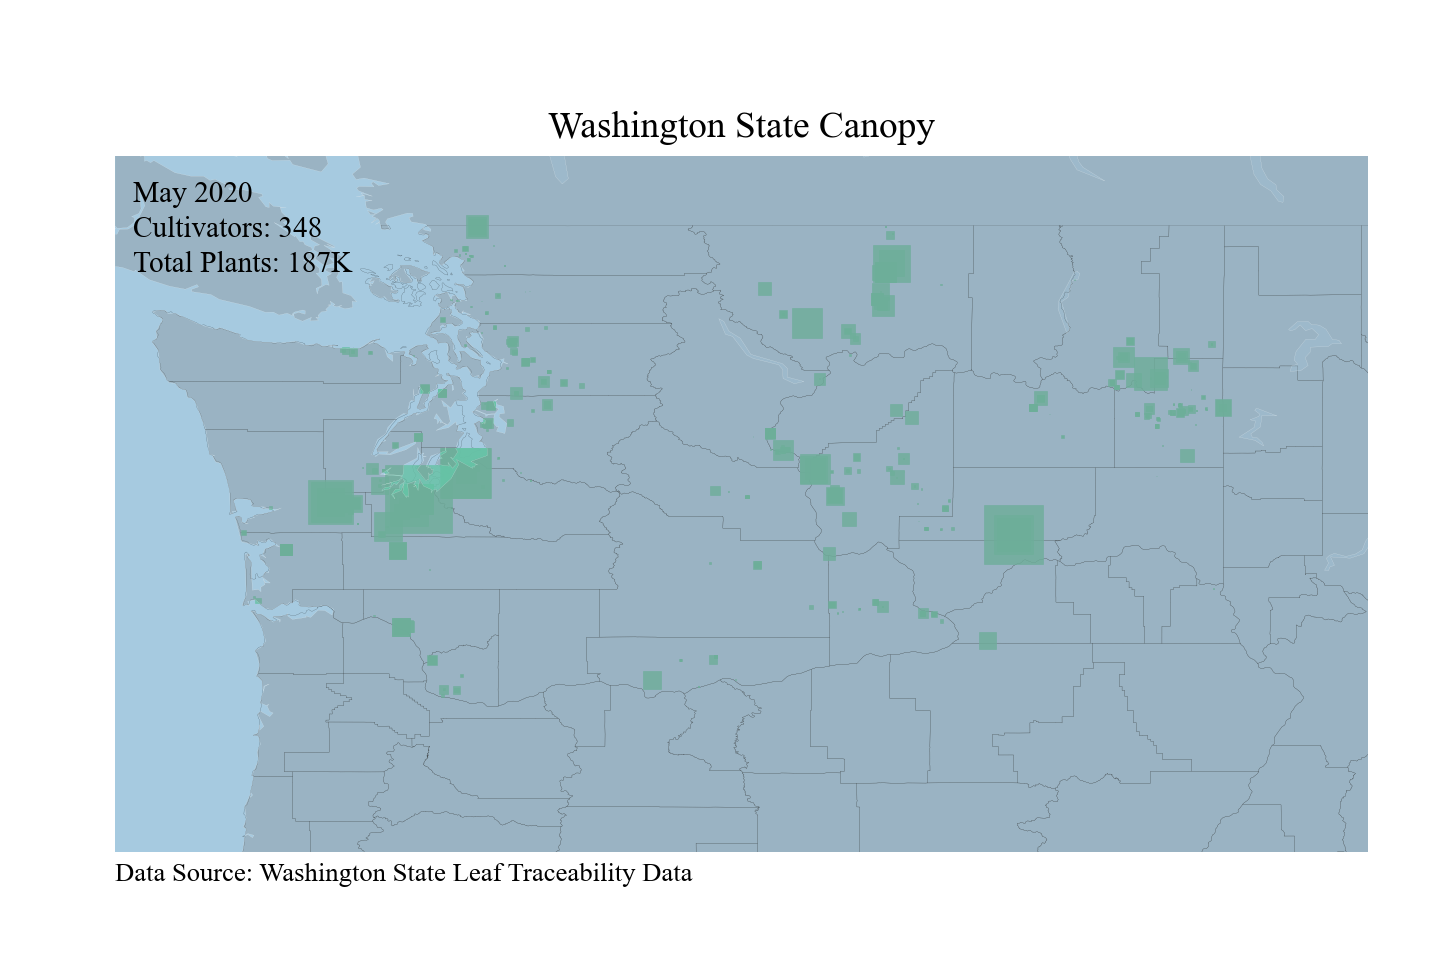
\includegraphics[width=\textwidth]{images/canopy-2020-05.png}
  \end{figure}
\end{minipage}%
\begin{minipage}{.5\textwidth}
  \begin{figure}
    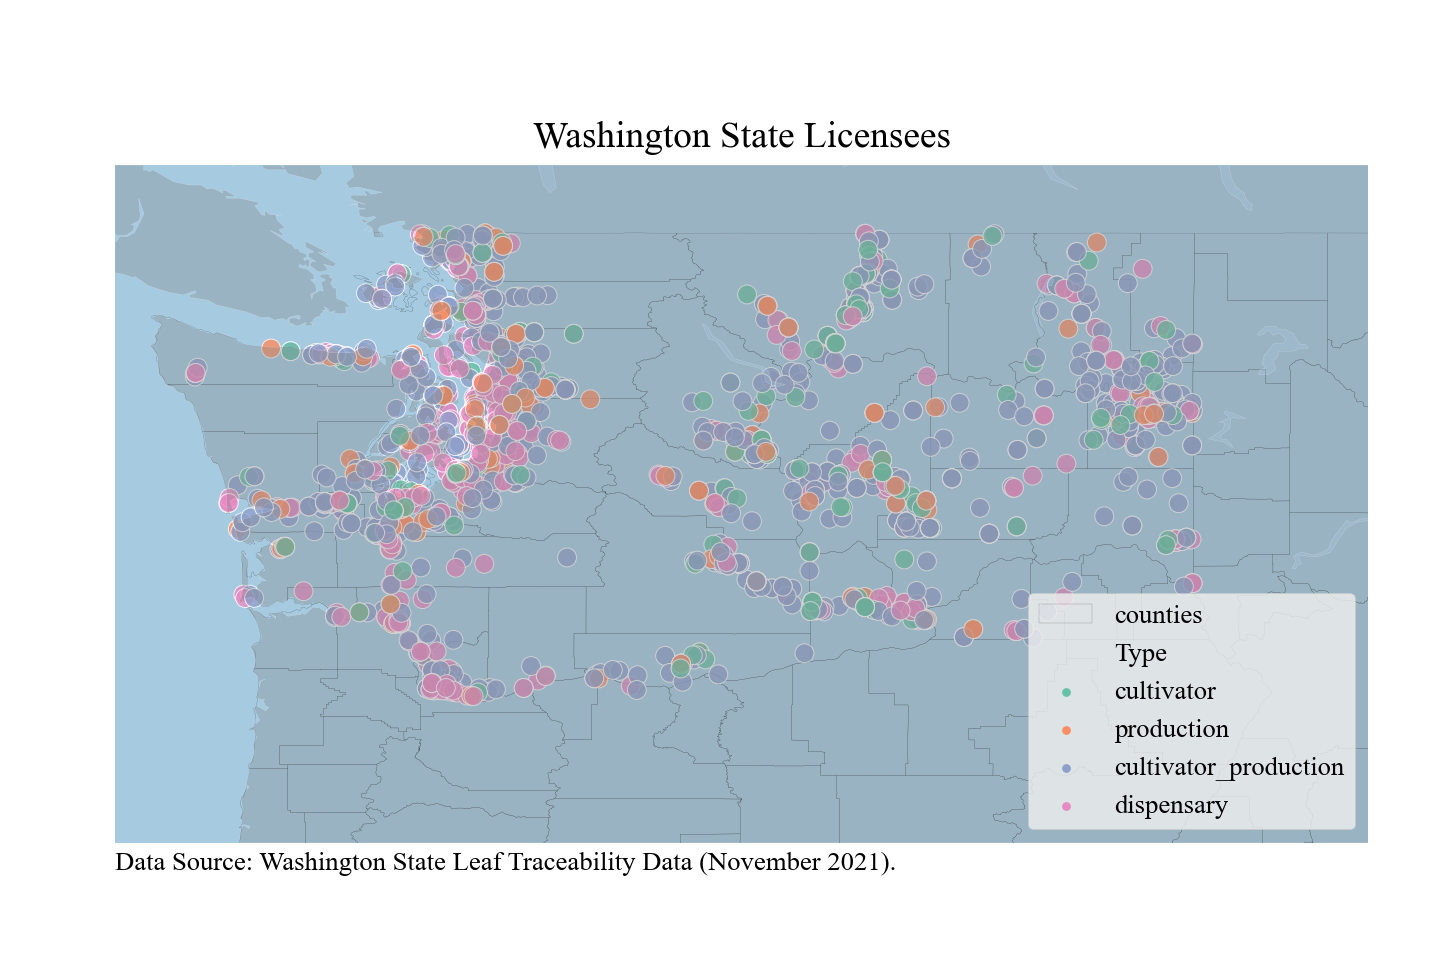
\includegraphics[width=\textwidth]{images/licensees_scatterplot.png}
  \end{figure}
\end{minipage}

% Question of the day
\begin{center}
\begin{minipage}{.9\linewidth}
\begin{Block}{Now The Question of the Day is Prices}

\vspace{.25\baselineskip}

Do cannabis prices vary by geography (zip code) in Washington State?

\vspace{.25\baselineskip}

\end{Block}
\end{minipage}
\end{center}

\end{frame}

%------------------------------------------%
% Spatial Analysis
%------------------------------------------%
\section{Spatial Analysis}

\begin{frame}{}

%\begin{center}
%{\large \textbf{Spatial Analysis}}\vspace{.5\baselineskip}\\
%\end{center}

Data maps (choropleths) were first used to visualize {\itshape moral statistics} on education, disease, crime, and living conditions.

% First Choropleth
\begin{figure}
  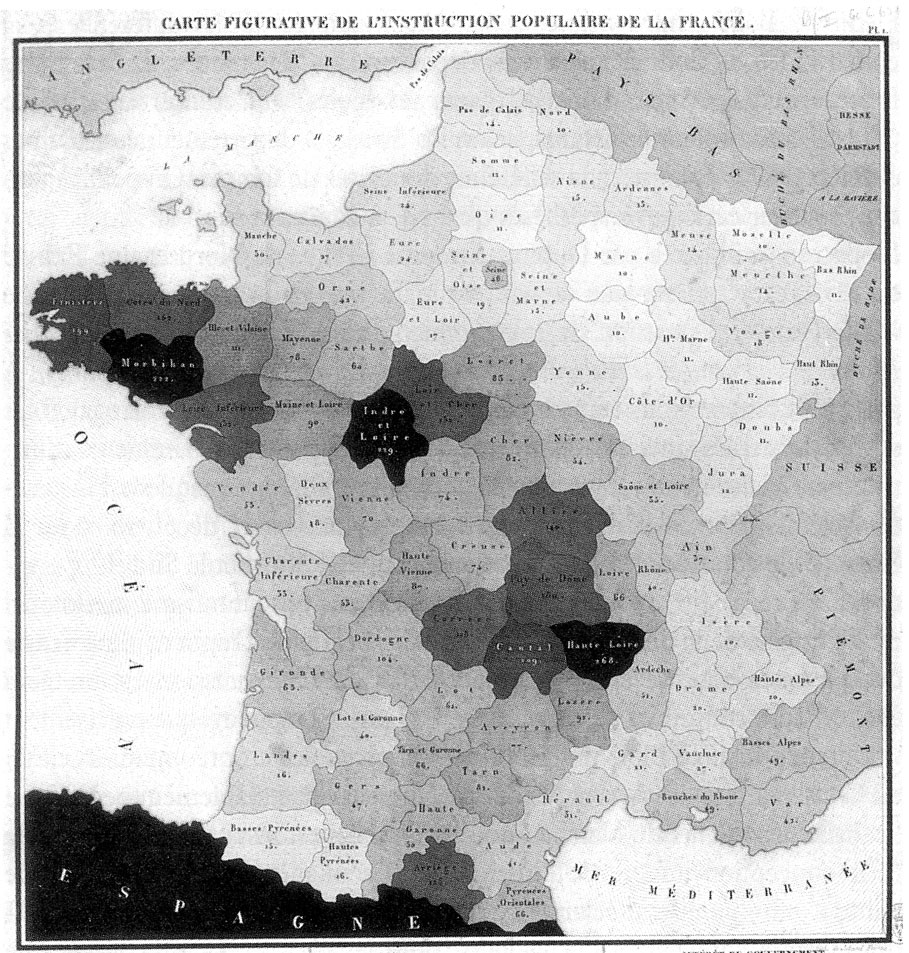
\includegraphics[width=.55\textwidth]{images/first-choropleth-france.jpg}
  \caption*{\footnotesize 1826 - The first choropleth, created by Baron Pierre Charles Dupin (1784-1873), depicts the availability of basic education in France by department.}
\end{figure}

\end{frame}

%------------------------------------------%
\begin{frame}{}

% Cholera Map
\begin{figure}
      \caption*{1854--1858 - A map created by Dr. John Snow (1813-1858) depicting cholera cases in the London epidemics of 1854.}
    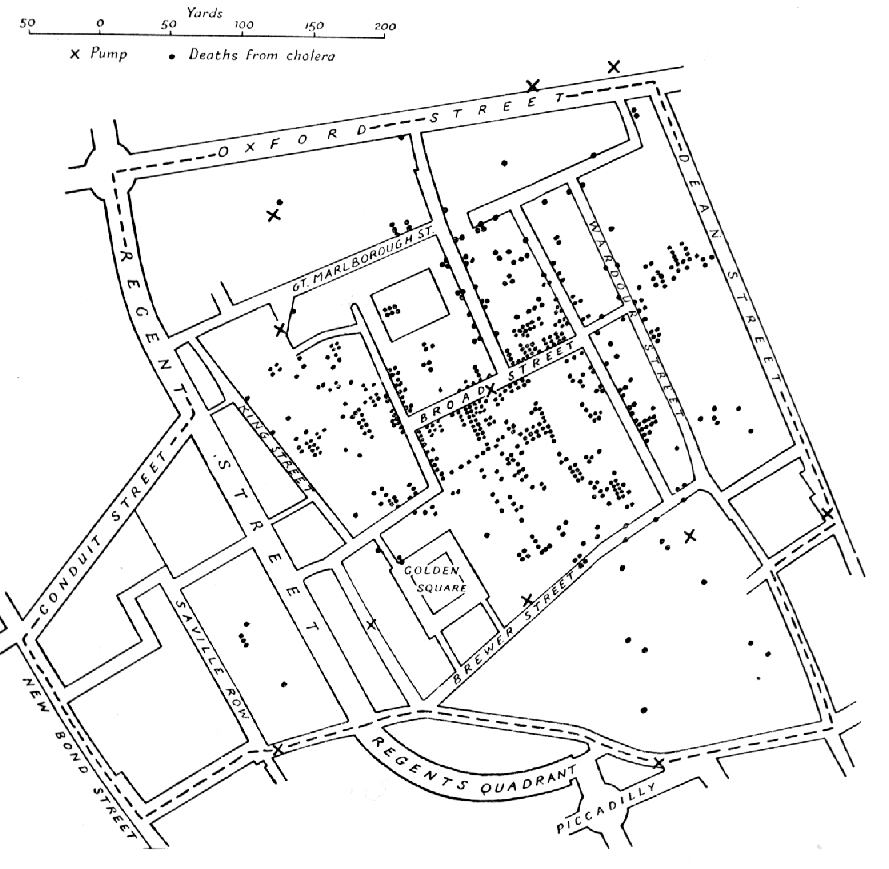
\includegraphics[width=.475\textwidth]{images/john-snow-cholera-map.jpg}
\end{figure}

{\footnotesize Fun fact: Dr. John Snow's research on cholera gave rise to the modern day difference-in-difference model\textsuperscript{1}.}

\vfill

{\tiny Designing Difference in Difference Studies: Best Practices for Public Health Policy Research\vspace{.25\baselineskip}\\Coady Wing et al., (2018).\vspace{-.75\baselineskip}\\https://doi.org/10.1146/annurev-publhealth-040617-013507}

\end{frame}

%------------------------------------------%
\begin{frame}{}

% Napoleon's March
\begin{figure}
  \caption*{1860 - Charles Minard depicts Napoleon’s 1812 Russia Campaign.}
  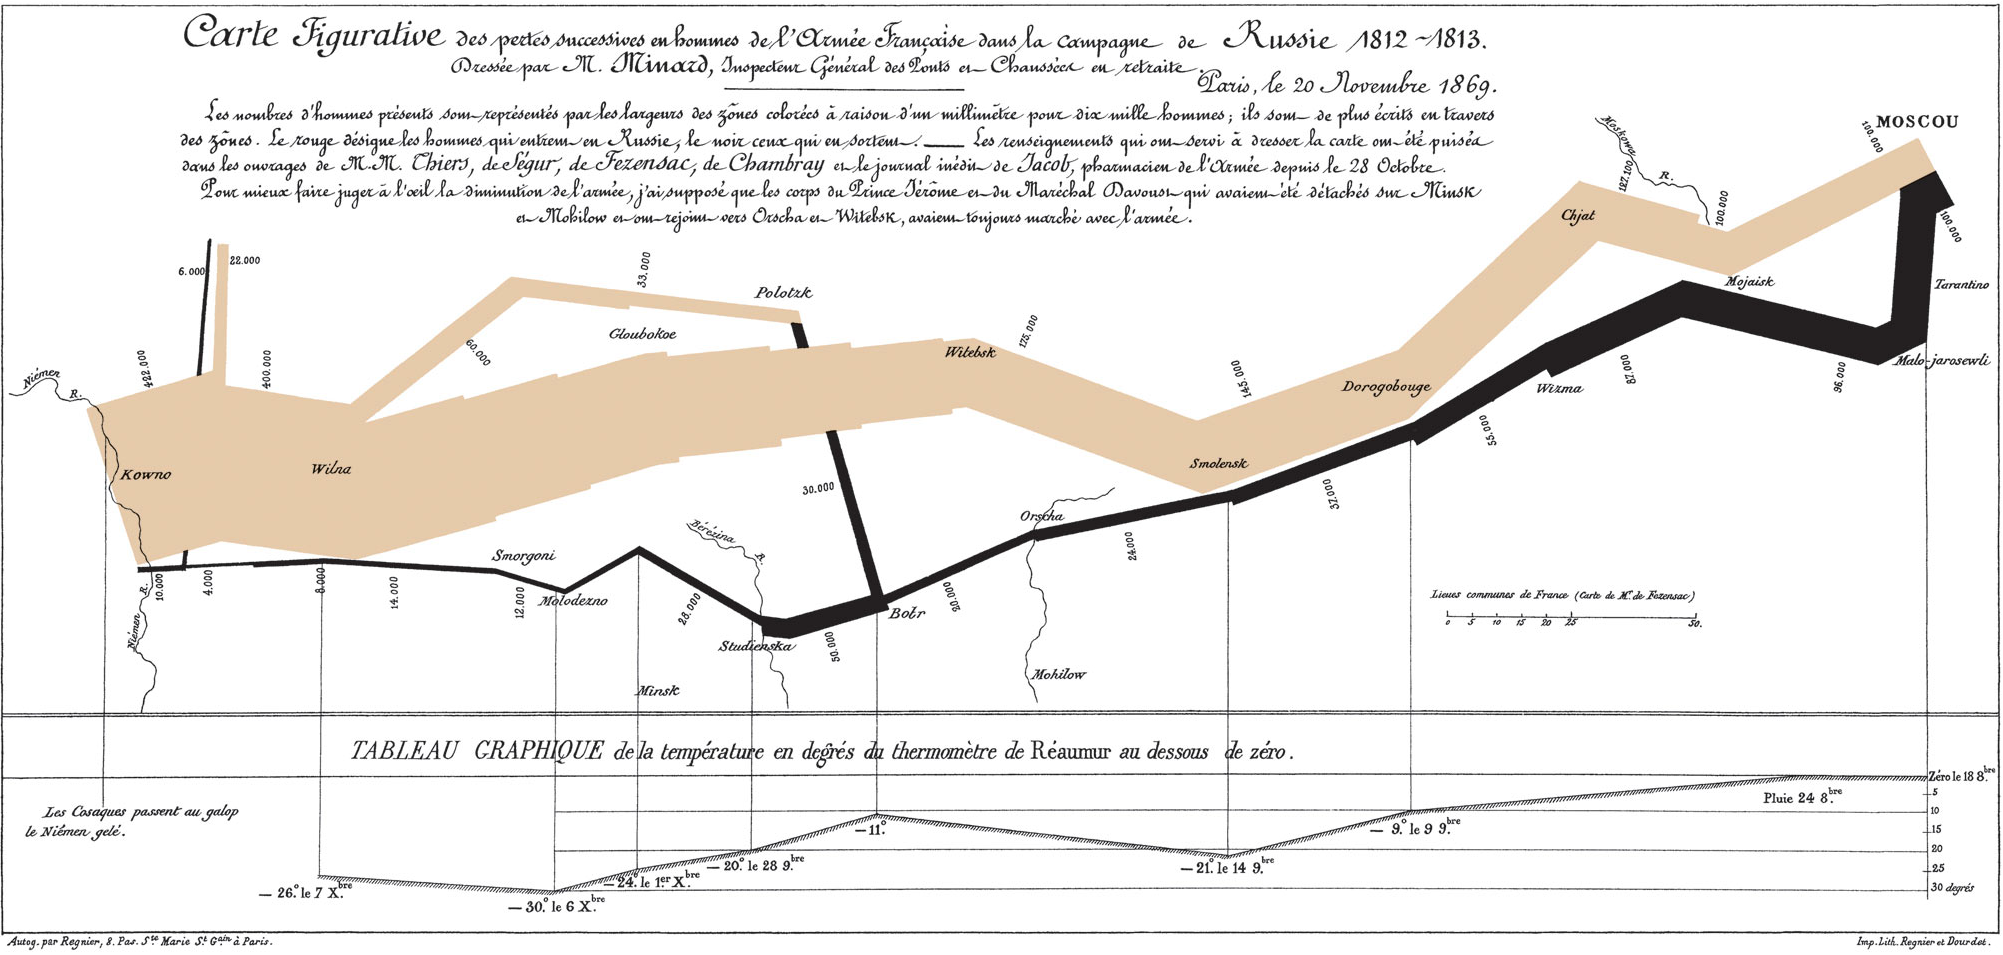
\includegraphics[width=\textwidth]{images/napolean-moscow-march.png}
\end{figure}


\end{frame}

%------------------------------------------%
% Choropleths
%------------------------------------------%
\section{Topics in Spatial Analysis}

\begin{frame}{}

{\large \textbf{Topics in Spatial Analysis}}\vspace{.5\baselineskip}\\

\begin{itemize}

\item Spatial dependence, autocorrelation, and association;

\vspace{.5\baselineskip}

\item Spatial interpolation;

\vspace{.5\baselineskip}

\item Spatial interaction, simulation, modeling.

\end{itemize}

  \begin{figure}
    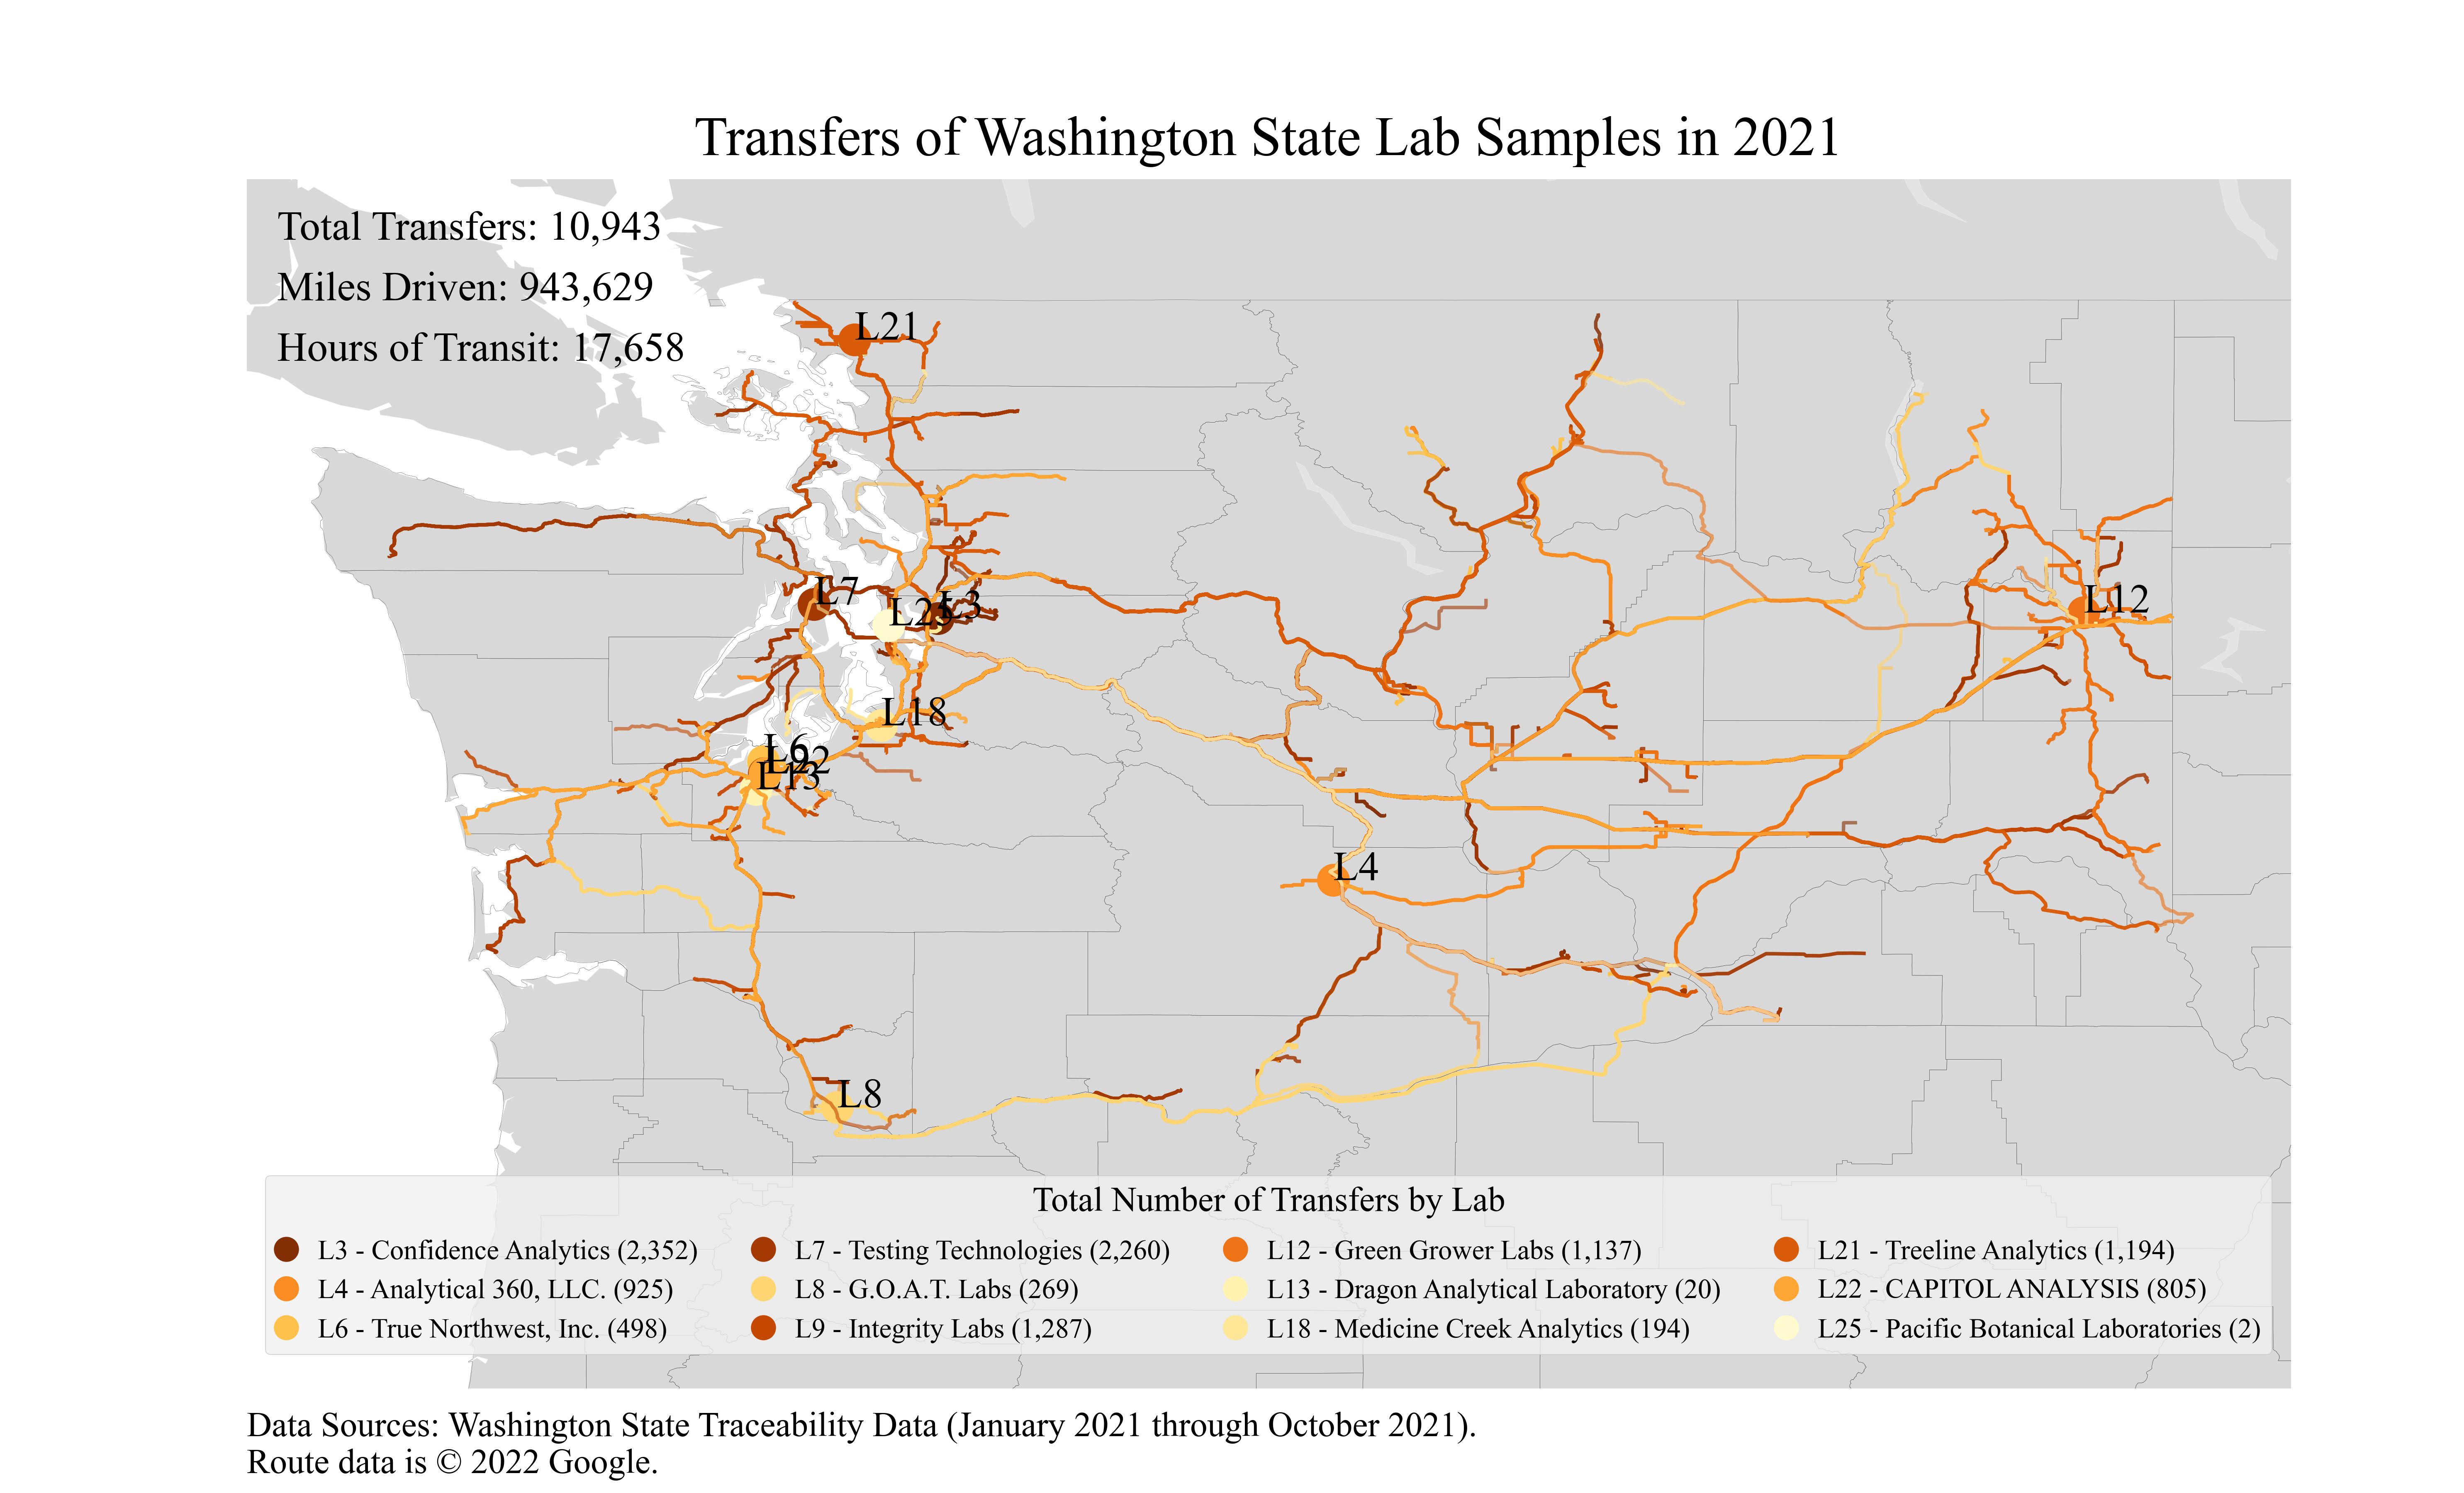
\includegraphics[width=.75\textwidth]{images/lab-transfers-2021.pdf}
  \end{figure}

\end{frame}

%------------------------------------------%
% Takeaway
%------------------------------------------%
\section{Takeaway}
\begin{frame}{}

\begin{center}
\begin{minipage}{3.85in}

% Thank you.

\includegraphics[width=.25in]{images/prayer.png} {\Large \textbf{Thank you for coming.}}\\

% Re-cap the lesson of the week.
\begin{center}
\begin{minipage}{.9\linewidth}
\begin{Block}{Lessons of the Day}

\vspace{\baselineskip}

\begin{itemize}

\item Visualizing data can help uncover insights that were hiding in plain sight.

\vspace{\baselineskip}

\end{itemize}

\end{Block}
\end{minipage}
\end{center}

\vfill

\end{minipage}
\end{center}

\end{frame}

%------------------------------------------%
% End
%------------------------------------------%
\end{document}
